\section{ADVERSARY DETECTION AND RED TEAM ASSET PROTECTION}
\label{sec:protection}
\glsresetall
The cyber red team has to maintain the visibility over the defended infrastructure and its own assets to ensure tracking of malicious activities, perform adversary assessment, gather further technical information aiding the attack trace-back and attribution, and protection of red team's operational infrastructure. Such detection and asset protection techniques benefit the cyber red team responsive operation execution and from the \gls{ooda} loop perspective they contribute to the observation and orientation actions.
Additionally, \gls{opsec} requirements have to be complied with to protect cyber red team assets, which are composed not only from the hardware and deployed software entities in cyberspace, but also the team identity and their operational goals.
Applicable techniques and solutions are presented in the listed publications (\ref{pub:fourthPub}, \ref{pub:fifthPub}, and \ref{pub:sixthPub}) and suitable use cases are assessed.

In contrast to a widely accepted belief, that attack is the best defence, the attackers might forget about defending their own assets and fail at insuring appropriate operational security measures. Such mistake can jeopardize the whole operation and lead to the full compromise of the cyber red team's infrastructure. This, most importantly, comes into consideration when the adversary is not only engaged in attacking the target infrastructure, but might pursue the defenders engaged in a responsive cyber defence. It has to be assumed that for every action there could be a counter action performed, thus leading to counter-red team operations and even to counter-counter-red team operations.
Defending party, executing a responsive cyber operation, is conducting operations from the infrastructure outside their defended network, which requires an equal and, in most cases, better protection. Such requirements stem from not only the threat detection perspective, but own asset, position, sensitivity of the pursued operational goals, infrastructure and identity protection requirements.

To provide such capabilities, the cyber red team has to have the expertise to implement, configure, supervise and monitor the threat detection solutions.
Such defence has to be implemented to cover the red team infrastructure's perimeter, as well as, activities happening within.
For the execution of crucial cyber operations the required red team environment would be custom made and deployed according to the operational needs, and afterwards securely destroyed.
To ensure such demands, the implemented defensive solutions have to meet at least the following criteria: readily-available, ease of deployment and management, flexible and scalable, high level of automation, and lightweight. Additionally, such solutions should be easily integrated with the technologies already present in the deployed network infrastructure elements, such as, \textit{rsyslog} or \textit{Syslog-ng} system logging services. Furthermore, these techniques, as well as the rest of the infrastructure, should be maintained to be as untraceable as possible and complicating the attribution. For such matters well developed, readily-available, non-commercial or open-source solutions providing high customization and flexibility would be applicable.
Two approaches complying with these requirements have been identified as system log (i.e., Syslog) based analysis and cyber deceptions.

In addition to automated syslog-based detection and cyber deception techniques, other threat assessment solutions can be used as well. Such solutions should comply with the mentioned criteria to be applicable for the cyber red teaming requirements. The proposed framework, named \textit{TED} (\ref{pub:ninthPub}), can be used on any modern GNU/Linux system with operating-system-level virtualization solution \textit{Docker} deployed. Foremost, such approach would be primarily used in the first stages of incident response on the systems, where no acceptable level of protection and threat detection solutions have been deployed or requiring additional in-depth assessment. \textit{TED} bundles most common local system and \textit{ELF} binary file security assessment tools, such as, \textit{checksec.sh}, \textit{Lynis}, and \textit{Spectre/Meltdown} checkers. All of the tools, their dependencies, management and orchestration scripts are included in a \textit{Docker} container, which can be used either in Internet connected or disconnected systems, and requiring only single requirement of \textit{Docker} engine being present. This engine is included in majority of the popular modern GNU/Linux distribution repositories and, in most cases, already being installed on systems, such as, application, and web servers. Such lightweight solution allows it to be easily used to establish system security level and identify potential binary file attacks, without introducing significant changes or requirement of installing other solutions on the target system, thus minimizing the contamination of the examined system. The potentially compromised system analysis has to be performed according to the digital forensics requirements, with assessing the system compromise likelihood and at least acquiring memory and disk images, before proceeding with more intrusive activities. Such activities may provide the needed situational awareness picture and assist initial technical attribution establishment, before engaging the specialized cyber red team into the computer network operations against a suspected actor in the cyberspace. Whenever the cyber red team moves from their defended information system into their operational infrastructure, from where the responsive operation will be carried out, the deployed assets in that infrastructure, in most cases, become disposable if deemed compromised. \textit{TED} may be used to assess the required hardening level of the initially deployed operational systems or in specific cases -- to examine the cause of their compromise. The primary solutions, compliant with the requirements and to be used within the defended and operational infrastructures, consist of system log file-based anomaly detection and cyber deception solutions.


\subsection{System Log File-Based Anomaly Detection}
System log file monitoring and analysis has been acknowledged as an important network and system management technique, as well as, granting the possibility of detecting anomalies and security violations.
Under normal circumstances, all network devices, such as, hosts, sensors, networking equipment or sophisticated data parsing and threat detection solutions, should be able to generate alerts and system logs in a textual format. It is highly recommended for such data to be delivered to a centralized storage location for retention, further analysis and correlation. Depending on the solution, the generated alerts and system logs can have a different representation, which might be parsed either without additional processing or requiring normalization or transformation to an unified standard. Despite this, easy to deploy and flexible system log processing and correlation method implementation into the cyber red team tool-set could grant the required visibility over the defended and protected assets.

Such system log file analysis should be performed for the defended network infrastructure, as well as, the operational one used by the red team.
Despite both environments collecting the log files, their design implementations could differ. Defended infrastructure could generate and record events in the log files, which are then transferred to the central location for retention and analysis, depending on the security policies and other requirements. The protected cyber red team operational infrastructure would follow similar approach, however, it might be beneficial not to keep the log files on the red team hosts or its supporting infrastructure, but directly delivered to the central secure location for immediate analysis and threat assessment. Such approach would be considered in case of a likely counter red team operation execution by the adversary and attacker possibly gaining access to the defending red team's infrastructure elements. This potentially could minimize the exposure regarding the executed responsive activities, intended goals and attribution.

Event correlation has established itself as a prominent and recognized monitoring technique, which is essential for establishing situational awareness.
The Simple Event Correlator (SEC) (\ref{pub:fourthPub}), written in Perl, runs on all modern UNIX based platforms, has been used for a wide range of purposes and environments as an efficient open-source alternative to the commercial solutions. This solution is designed for real-time event processing and incorporates event matching, parsing, and output generation.
The SEC uses scalable rules for event correlation, which can be applied to a range of inputs, including the Syslog files.

This lightweight, flexible and real-time nature of SEC complements the cyber red team operational requirements, allowing focus on the operation itself while gathering and receiving real-time alerts. Such visibility, enhanced by the user interface such as \textit{Kibana} from the \textit{ELK Stack}, can deliver the required situational awareness regarding the cyber red team's operational infrastructure. Gained awareness not only allows pinpointing the system failures or monitor the infrastructure performance, but allows to detect anomalies, such as, attacks or unsanctioned access attempts.

Despite the SEC being powerful event correlation solution, it relies on its rule-sets, which have to be created by the human analyst.
A novel data mining-based framework is developed (\ref{pub:fifthPub}), requiring no human intervention, for fully automated rule discovery for real-time detection of anomalous messages from Syslog-based logs. This approach possesses the capability to adapt to the changes in the system and employs the \textit{LogCluster} algorithm for data mining.
Human expert can extend the framework with own created rules, thus aiding the anomaly detection or adjusting the system to the specific design implementation or operational goals.

The detection of previously unknown error conditions and anomalies has been a difficult problem, however, the proposed framework provides a one practically applicable solution to it. The cyber red team implementing this solution on the centralized Syslog collector, to which the individual host system logs are transferred over a reliable and encrypted channel, gains an immediate benefit with least efforts required.
As the conducted experiments over a larger period of time have indicated, the anomalies and unexpected system state conditions have been successfully identified. Furthermore, the test involving the running of \textit{Bbuzz} fuzzing framework for abnormal network communication generation, clearly confirms that unknown anomalous or malicious requests, resulting in the Syslog entries, are detected and reported.
It has to be noted, that cyber red team protected operational infrastructure should implement also the traditional defensive mechanisms (i.e., passive defence), such as, packet filtering on all network hosts (e.g., \textit{iptables}, \textit{ip6tables}, \textit{Firewall \& network protection}), deploy proper system hardening (e.g., \textit{SeLinux}, application white-listing), host protection with \gls{hids}, system disk encryption (e.g., \textit{LUKS}, \textit{BitLocker}, \textit{VeraCrypt}), and user privilege level separation and control. When deploying the defensive measures, they have to be assessed from the operational security considerations to confirm, that no information is leaked out from the infrastructure to the third parties, such as, anti-virus, \gls{hids} or \gls{ids} alerts and metrics.
When considering a potential counter-red team operation executed by an adversary the similar attack approaches have to be expected and system protection should be augmented by the out-of-band (e.g., hardware or software-based port mirroring) network traffic monitoring and analysis solutions, such as, \textit{Snort}, \textit{Suricata} and depending on available resources and team capabilities -- \textit{Bro} and \textit{Moloch}. These solutions in turn would also generate the alerts and system logs, which can be transferred to the central location for the data mining, correlation and security incident information extraction.
If the cyber red team assumes the high risk of the counter-red team operation plausibility, then further in-depth system monitoring solutions can be considered for deployment to deliver additional visibility, such as, system performance metrics (e.g., \textit{sysdig}, \textit{Telegraf}), kernel requests (e.g., \textit{Snoopy}), unsanctioned system use (e.g., \textit{tripwire}).


\subsection{Cyber Deception-Based Detection}
All of the presented passive monitoring and threat detection techniques should be augmented with the active cyber defence elements within the cyber red team's operational infrastructure.
The most prominent one, as described in the chapter \ref{sec:rcd-work}, has been identified as the cyber deception approach.
If deployed either in the defended system or in the protected cyber red team operational network this set of techniques would grant the immediate feedback to the cyber red team on any identified suspicious activities.
Cyber deceptions can further be integrated to deliver their system logs and alerts to the central Syslog processing location.
Various types of cyber deceptions can provide different levels of adversary tracking and technical attribution information gathering. The solutions, such as honeypots, would be able to identify unsanctioned access to them and collect information on adversary's activities within the decoy network allowing a better insight into their capabilities, intentions and \gls{tttp}.
Honeytokens could potentially allow the trace-back to the location from where such data has been executed or accessed.

The following cyber deception frameworks were implemented in the reference network, against which the targeted attacks were launched (\ref{pub:sixthPub}) -- \textit{T-pot}\footnote{DTAG Community Honeypot Project. \url{http://dtag-dev-sec.github.io/}. Accessed: 05/10/2018}, SHIVA\footnote{Spam Honeypot with Intelligent Virtual Analyzer. \url{https://github.com/shiva-spampot/shiva}. Accessed: 05/10/2018}, YALIH\footnote{Yet Another Low Interaction Honeyclient. \url{https://github.com/Masood-M/yalih}. Accessed: 05/10/2018}, KFsensor\footnote{Advanced Windows Honeypot System. \url{http://www.keyfocus.net/kfsensor/}. Accessed: 05/10/2018}, and ADHD (see footnote \ref{fnote:adhd} on page \pageref{fnote:adhd}).
To conduct the experiments the target network consisted of various zones, such as, demilitarized network hosting external web and e-mail services, internal network for business purposes hosting MS Windows and GNU/Linux clients, and a sub-net for information system security monitoring solutions. Every sub-net represents location for deployment of an applicable cyber kill-chain technique both from the attacker and the defender perspectives. The cyber deceptions, according to their applicability and expected use cases were deployed in the network segments to match the defender's requirements on stopping the attack according to the cyber attack kill-chain stages.
Every particular framework or a collection of tools is either oriented towards being deployed on its own client operating system (e.g., GNU/Linux, MS Windows), is a high- or low-interaction honeypot oriented at deceiving the adversary or is a set of tools to be used to actively detect, counter or degrade the attacker's capabilities (e.g., port-spoofing, \textit{tarpit}). The experiment results identified, that out of all implemented technologies the multi-honeypot platform \textit{T-pot} proved to be the most efficient in identifying and detecting attack or malicious activities. \textit{T-pot} includes a set of \textit{dockerized} instances of multiple solutions, such as, \textit{Glastopf, Kippo, Honeytrap, and Dionaea} honeypots, \textit{Suricata} \gls{nids}, \textit{ELK} stack, and \textit{ewsposter} for honeypot data sharing.
The cyber deception is a valid method for detecting, deceiving, disrupting, degrading, denying, and defending against the adversary.

\textit{Detect}. As this being one of the core requirements for any defensive activity, it is required to establish the situational awareness and allow pursuing responsive activities against the detected threat. All of the mentioned passive methods and further described active ones, contribute to achieving this goal. To complement attribution via the active detection means, the most prominent approach could be various cyber deception techniques, such as, \textit{honeytoken} documents rigged with an executable code, or strategically placed decoy data leading the attacker to the deployed honeypots. Rigged documents, such as, attack orders, technical documentation, or other sensitive information, once exfiltrated from the defended infrastructure and opened by an attacker potentially could reveal the adversary position in the cyberspace by \textit{beaconing} its IP address and other sensitive data collected and sent by the embedded computer code. Depending on the adversary's operational security methods, such as, rigged files might be either stripped of executable scripts, opened on an isolated or third-party system, or modified to deliver false information. Despite these concerns, this option should be practised by the cyber red team to raise the level of attribution in case the cyber deceptions are well crafted and placed or if the adversary is careless and makes a mistake.

\textit{Deceive}. Part of defensive activities, especially ones implemented in the cyber red team's operational infrastructure, should be aimed at confusing and deceiving the adversary by any means possible. The techniques, such as, decoys and cyber deceptions will not only allow the identification and tracking of the adversary, but would also allow its attribution, technical capability and goal assessment. The concept of cyber deceptions would include solutions, such as, honeypots which would spoof the attack surface by deploying large quantities of simulated hosts or network topologies (i.e., honeynets). Besides providing deception this technique also supports the degradation of attacker capacity, since adversary would be entangled in sorting identified systems between the real and fake ones. Both low- and high-interaction honeypots benefit the attribution process, additionally granting the insight into adversarial \gls{tttp} in case of a high-interaction honeypot usage. It has to be noted, that high-interaction honeypots might require a larger effort for maintenance and upkeep in contrast to the low-interaction ones but would also give a better understanding of the adversarial objectives and motivation. However, it would be highly suggested to have at least the low-interaction honeypots embedded in the red team's infrastructure.
To further control and deceive an adversary decoys could be placed throughout the red team's operational infrastructure. The strategically placed decoys (sometimes called ``breadcrumbs''), for example, in the form of cached credentials, saved remote connection sessions or mapped network drives, would try to force the attacker use this seemingly valuable information to follow the predefined path designed by the defender leading to a decoy system. Once this decoy information is used against the decoy system (e.g., honeypot), the alert is triggered, and further perpetrator actions can be monitored and traced. One of the rising solutions in providing such cyber decoy systems based on sophisticated scenario development, ``breadcrumb'' creation and placement is the \textit{Mazerunner} (see footnote \ref{fnote:mazerunner} on page \pageref{fnote:mazerunner}).

\textit{Disrupt}. If a detected and identified attack becomes too intrusive or tries to overwhelm the protected infrastructure, it is possible to disrupt the connections either by firewalling or \textit{null-routing} them. Such action does not directly aid the attribution or adversary assessment, however, can be used to indirectly limit available attack paths thus potentially steering the perpetrators towards the desired communication channels or approaches which can be controlled or monitored by the cyber red team. Depending on the situation, it might be chosen not to disrupt the adversary activities within the protected networks, but to carry on observing and analysing them to gain more intelligence information on the threat actor.

\textit{Degrade}. Any active or responsive action depends on time, thus deception and degradation approaches are used for the defenders to gain additional time to respond while opponent is being tricked in performing useless activities. Degradation by inflicting the time penalty is typically executed by at least the following approaches -- honeypots to artificially increase the network complexity and size for the attacker to spend time on probing it, network host attack surface spoofing to force attacker wasting time on performing endless network port scans, and \textit{tarpitting} incurring a serious time cost when dealing with slowly responding services to all requests. In some cases, degradation would be seen as better approach instead of disrupting, due to the fact that the adversary will still attempt to invest time instead of leaving or searching alternatives.
In cases when active engagement against enemy communication channels or capabilities is executed, the opponent will comprehend that they are being deceived or caught and might change their tactics and approaches. Depending on the situation this might be desirable to observe the true potential and capacity of the threat actor.

\textit{Deny}. If disrupt and degrade are active engagements against already ongoing attack and its paths, the denial would proactively assess and anticipate attacker's goals and eliminate the attack paths even before they are pursued. This could be linked together with detection and deception techniques, where adversary presence and goals are identified and isolated to limit their movement within the defended network. For such option to be feasible, all of the infrastructure hosts should be centrally manageable through the solution, such as, \textit{Salt} stack. However, if such central management solution is taken over by the adversary then the cyber red team could potentially lose all their assets and the operation becoming fully compromised.

\textit{Defend}. The overarching concept merging all of the individual approaches to provide the unified goal for guarding either the defended information systems or protecting the red team's assets and operational infrastructure.


\subsection{Cyber Red Team Operational Infrastructure Protection Considerations}
\label{sec:opinfra}
The proposed conceptual model for cyber red team's operational infrastructure (Fig. \ref{fig:rtinfra}) consists of multiple logical network zones, designated by their purpose and usage. This comprehensive infrastructure model is just one of the possible variations, and will be dependant on the operational requirements, resources and time available. The figure represents the infrastructure concept design, functional area purpose and host description, and deployed defensive measure applicability. The key factor in this operational network prototype is to assess which of the described and researched techniques and tools for the detection and deception are applicable and in what ways.
This cyber red team operational infrastructure model has been implemented to a certain extent in the technical cyber exercise ``Crossed Swords'' and is covered in more details in chapter \ref{sec:xs}.

From the previously assessed approaches on Syslog-based anomaly and cyber deception based detection, the following techniques are considered: 
\begin{enumerate}
    \item \textit{passive defence}, supporting defend, disrupt, and deny activities, focuses on host and network device hardening, packet filtering, \gls{nids}, communication channel redundancy, security and encryption, and network segmentation;
    \item \textit{Syslog analysis}, supporting detect activity, aims at anomaly and threat detection by analysing aggregated system log and alert information from the network nodes;
    \item \textit{Attack surface spoofing}, supporting degrade and deceive activities, is a form of cyber deception for spoofing a large attack surface to confuse and stall the adversary;
    \item \textit{honeypot}, supporting deceive, degrade, and detect activities, is a form of active threat detection and can be used for adversary activity tracking, attack surface spoofing (e.g., honeynets) and stalling the movement of attacker within the network;
    \item \textit{cyber decoy}, supporting deceive, degrade, and detect activities, is a form of a decoy, such as, the ``honeytoken'' or ``breadcrumb'' information deployed on network hosts, to lure the adversary towards a detection system (e.g., honeypot) or to reveal its current position in the cyberspace (e.g., beaconing); and
    \item \textit{tarpit}, supporting degrade activity, directly aims at stalling the incoming attack progression by responding slowly to received requests.
\end{enumerate}

\begin{figure}[!htb]
    \centering
    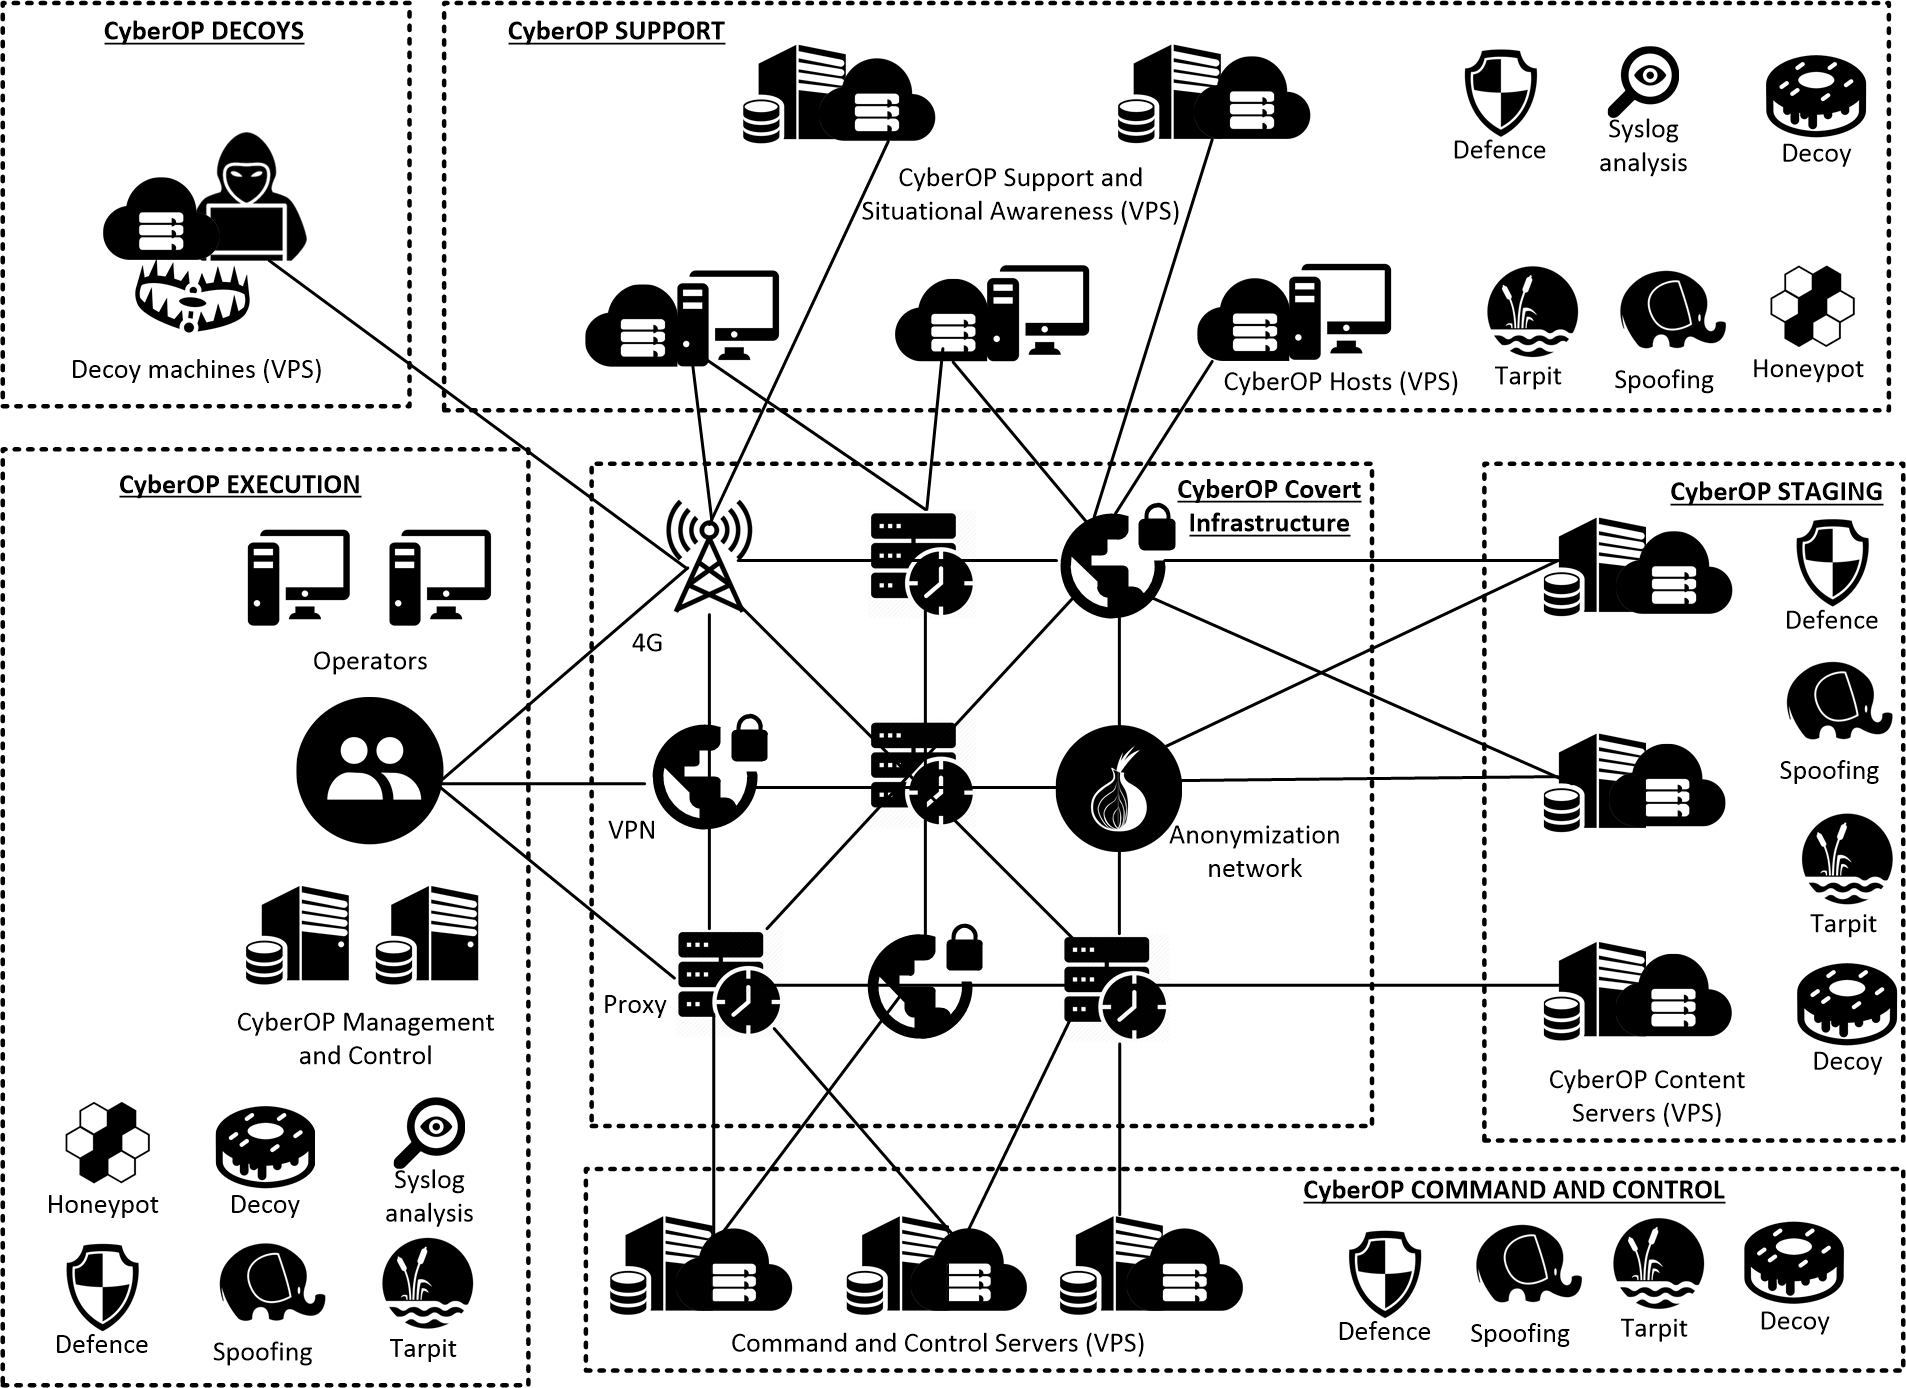
\includegraphics[width=1.0\textwidth]{./img/crt_infra.jpg}
    \caption{Cyber red team operational infrastructure concept model and defence measures}
    \label{fig:rtinfra}
\end{figure}

Cyber operation covert infrastructure is a set of interconnected nodes on the Internet by the use of various communication technologies, such as, mobile 4G data connections, VPN tunnels, proxy servers, connection bouncers, or anonymization networks (e.g., TOR, i2p). The purpose of the covert infrastructure is to ensure the maximum possible un-traceability to the origin of the cyber red team operators connecting to their deployed assets in the cyberspace. Depending on the operational requirements, at least two network hops should be taken. Relying upon the design of such covert network, the interconnections between the nodes can be changed dynamically whilst maintaining and ensuring the overall connectivity between the two or more interconnected nodes or groups of nodes engaged in the cyber red team operation.
Various design approaches can be chosen and implemented to design the overall cyber red team infrastructure and divide it in logical groups basing on their purpose and usage. This might depend on various factors, such as, if a particular adversary \gls{tttp} are impersonated for the ``false-flag'' operations, complexity and sensitivity of the performed computer network operations, available resources, and if the cyber red team wants to expose the advanced capacities and capabilities it possesses. For example, a covert network for a high value computer network operation aiming at executing a sophisticated targeted attack against adversary information systems and establishing a \gls{cnc} control over the compromised nodes, might have the following architecture requiring applicable defensive measures (Fig. \ref{fig:rtinfra}):
\begin{enumerate}
    \item Cyber operation execution area, where the cyber red team is located and the connections to their assets in cyberspace over the covert infrastructure is established. This \textit{home} network would host not only the computer systems from which the operation is originating, but also supporting systems, such as, the situational awareness provision, operation tasking and organisation, collected information cataloguing, indexing and management, operational network supervision, testing, research and development systems, and covert infrastructure automated creation, administration, adaptation and destruction.
    In this area all of the protection techniques, passive defence, Syslog analysis, spoofing, honeypots, cyber decoys, and tarpits, are applicable to provide maximum possible defence for the cyber operation origin and execution orchestration;
    \item Cyber operation support area, where hosts engaged in conducting and supporting the computer network operation are located. All of the nodes are automatically deployed, hosted and afterwards securely destroyed (e.g., overwriting the encrypted file system with random data, such as \textit{/dev/urandom}) on a purchased \gls{vps} operator infrastructure. These nodes are supported by the deployed \gls{vps} systems, such as, operational infrastructure supervision, Syslog aggregation and analysis, and secured immediate operational information storage.
    The same protection mechanisms as for the cyber operation execution area are applicable here as it is a vital set of assets on which the success of the operation depends;
    \item Cyber operation staging area hosts the exposed \gls{vps} nodes engaged in delivering or hosting the attack artefacts. This would include systems, such as, SMTP servers for sending e-mails to the target, web servers for hosting the malware and dive-by exploitation kits, and target network reconnaissance tools. These hosts are used for direct interaction with the adversary for activities, such as, reconnaissance or initial foothold establishment. Taking into account that these systems, due to the nature of their usage, can be identified by the target, a pool of active and stand-by systems are required to be changed once they have been discovered or have fulfilled their intended purpose.
    Furthermore, this area can include not only the assets deployed by the cyber red team on the public \gls{vps}, but also any other public or cloud-based solutions, for example, \textit{Dropbox} for hosting malicious payloads, \textit{Google docs} end for credential harvesting, and \textit{Twitter} feed for \gls{cnc} command issue. Such public service utilization raises the level of scalability, set-up and destruction, minimizes the expenses and time investment, as well as benefits to raising the level of anonymity.
    This group of assets due to their high exposure nature and direct engagement with the target have to possess a set of protection mechanisms allowing to estimate asset compromise and tracking of adversarial activities. The techniques, such as, passive defence, spoofing, tarpitting, and decoys, are applicable to ensure a decent level of protection, however, without having a straightforward link, even using covert infrastructure, back to the cyber operation support area. Instead decoys would try to lure the attacker towards the cyber decoy area \gls{vps} hosts instead, which then would report any detected activities back to the cyber support area servers. Varied choice for protection technique tools and implementations should be employed across all protected assets to limit the cyber infrastructure host fingerprinting and identification within the cyberspace based on the defensive and techniques in use;
    \item Cyber operation command and control area is the set of \gls{vps} based nodes hosting the \gls{cnc} \gls{vps} servers. Upon a successful attack from the cyber operation staging area, the compromised hosts are designed to call back to the intended \gls{cnc} servers. The connection to the \gls{cnc} servers is handled via the redirectors in the cover infrastructure, thus limiting the direct exposure of this critical asset. However, the possibility of their detection and targeting by the adversary exists, therefore a set of active and hot stand-by \gls{cnc} servers is required to transfer the control from one to another in case one has been identified or compromised.
    Exactly the same protection considerations are applicable to this area as for cyber operation staging hosts due to the high exposure and direct interaction with the target information systems; and
    \item Cyber operation decoy area is the landing area to where the stored decoys would attempt to lure the adversary, which is trying to take control over the cyber red team assets and tracing back to the origin of attack. This area would host nodes, such as, honeypots, and sensors for \textit{honeytoken} beacons. The detected interactions with these decoys would be logged and sent to the cyber operation support area servers, such as, Syslog collection and analysis.
    In this area, systems, such as, the honeypots, decoy destination, and beaconing detectors, are deployed. Since these hosts are designed for actual interaction with the adversary, it would be advisable for them to be designed to look as legitimate as possible to make the attacker believe that some actual cyber red team operational hosts have been reached and thus reveal their position and \gls{tttp}. However, still having some level of hardening implemented to deny full compromise of the hosts. Depending on the cyber operation infrastructure goals, the high- and low-interaction honeypots or a mix of both could be implemented, taking into consideration, that high-interaction systems, in comparison to low-interaction ones, would deliver a more believable experience, but demand higher maintenance and can be potentially fully compromised. Adaptive self-configurable honeypots \cite{Wagener2011} \cite{Zhang2017} allowing the adjustment to the incoming attack to provide the highest possible level of interaction and experience for tracking the adversary and permitting to perform threat assessment.
\end{enumerate}
Author acknowledges that \gls{ai} technologies, such as, artificial neural networks and machine learning, should be considered for cyber red team operational network design, implementation and protection.
Also, the MITRE ATT\&CK and PRE-ATT\&CK \cite{MITRE-ATTACK} can be considered for cyber red team \gls{opsec} requirements and when being engaged in false-flag operations with particular threat actor's \gls{tttp}.
Furthermore, the protection has to be ensured for cyber red team obtained and controlled assets, such as, DNS names, virtual private servers, bullet-proof hosting services, social network profiles, \gls{osint} tools (e.g., Shodan, Maltego, VirusTotal \gls{api}), cloud services (e.g., MS Office 365) and payment methods. However, such protection mechanisms would more revolve around using privacy and anonymity ensuring services, use of covert infrastructure for their access, have unique accounts and associated registration data, payments by hard to trace methods (e.g., crypto-currency, )

\subsection{Chapter Conclusions}
This chapter examines the use and applicability of the detection and deception solutions for integration into the cyber red team life-cycle and asset protection. The described novel log-based anomaly detection approaches (\ref{pub:fourthPub}, \ref{pub:fifthPub}) and existing cyber deception solutions (\ref{pub:sixthPub}) deliver the required effects to benefit the \gls{crt} conducted operations, such as, adversary tracking, threat assessment, technical attribution, red team asset protection, \gls{opsec} improvements, and situational awareness. While conducting the responsive computer network operations the \gls{crt} has to bear in mind, that the pursued adversary might engage in the counter-red team activities, thus endangering the not protected \gls{crt} assets and jeopardizing the whole responsive operation. Additionally, solutions, compliant with cyber red team operational requirements, can be used for initial response to confirm the defended system security breach and gather initial technical attribution information (\ref{pub:ninthPub}).
The proposed concept model for the cyber red team operational infrastructure (Fig. \ref{fig:rtinfra}) displays and explains the reasoning and benefits of the detection and deception methods deployed therein. Such model, if adapted and customized according to operational requirements, would provide the necessary situational awareness, increased stealth, and benefit to gaining advantage over the adversary.